\renewcommand{\partname}{}
\renewcommand{\chaptername}{}
\renewcommand{\thechapter}{}
\renewcommand{\thesection}{}

\chapter{Anonymisation des données}
\subsection{Qu'est-ce que l’anonymisation?} 

l’avis du G29\footnote{Groupe de travail institué par l’article 29 de la directive 95/46/CE. Il s’agit d’un organe consultatif européen indépendant
sur la protection des données et de la vie privée. Ses missions sont définies à l’article 30 de la directive 95/46/CE et à l’article
15 de la directive 2002/58/CE.}[4] rappelle que \textbf{\emph{l’anonymisation}}, au sens de la directive 95/46/CE (abrogé par le règlement numéro 2016/679 dit \gls{RGPD})
\begin{em}
    "est le résultat du traitement des données personnelles afin d’empêcher de façon irréversible, toute identification"
\end{em}  

L’anonymisation est donc ce processus qui supprime tout lien directe ou indirecte entre une personne et la donnée qui la concerne. Mais le défi majeur de l’anonymisation réside dans le fait de pouvoir garder l’utilité de l’information que contient une donnée.  En effet, plus on cherche à anonymiser plus grande est la perte de l’information.  
Ainsi donc, l’anonymisation et la re-identification ont fait et font toujours l’objet de plusieurs études. Certains cherchent des techniques de plus en plus performantes pour rendre anonyme, d’autres, des techniques pour casser les techniques précédentes. Nous citerons l'exemple de Lantanya Sweeney, qui, au début des années 2000, prouva qu’une méthode (appelé aujourd’hui pseudonymisation) n’était pas efficace pour anonymiser et   proposa une autre méthode nommée k-Anonymat, ([5], que nous verrons plus tard. 

\subsection{Différence entre l’anonymisation et la pseudonymisation}

Le caractère irréversible doit être établie pour dire qu’il y a anonymisation. Dans le cas contraire il s’agit d’une pseudonymisation. Nombreux sont ceux qui confondent l’anonymisation et la pseudonymisation. Ce dernier, se dit d’un processus qui remplace un attribut (généralement un attribut unique) par un autre (appelé pseudonyme) dans un enregistrement [6, p. 29]. 

L’avantage de la pseudonymisation est que tant qu’on ne traite pas les champs identifiants, les résultats sur les autres champs sont identiques que des résultats effectués sur une base non anonymisée. Toutefois, la pseudonymisation reste fragile aux attaques de type record linkage, mis en évidence par Latanya Sweeney. Elle put identifier une partie des individus issus d’une base de données médicale (pseudonymisée) croisée avec une liste électorale publique. 

\subsection{Pourquoi faut-il anonymiser?} 

L’objectif principale de l’anonymisation est de réduire à un niveau acceptable le risque de réidentification. Il faut anonymiser car, des règles de confidentialité et de sécurité sont imposés par la loi surtout quand il s’agit de données personnelles. Ces lois sont là pour empêcher des tierces personnes à accéder à des données personnelles [7]. 


\subsection{Quand faut-il anonymiser?} 

S’il est évident qu’il est nécessaire d’anonymiser dès lors que des données (à caractères personnels) quittent un environnement sécurisé pour être rendus publique, il convient aussi d’anonymiser les données dès leur processus de réception. Ce deuxième cas, suppose que le risque zéro n’existe pas et, qu’aussi sécurisé soit-elle, une base de données peut toujours tomber aux mains d’une personne malveillante. 

Ainsi on distingue deux stades pour l’anonymisation: 

L’anonymisation à bref délai: les données collectées sont tout de suite anonymisées (dans un délai allant de quelques secondes à quelques minutes). Le responsable de traitement à l’obligation d’indiquer son identité et la finalité du traitement pour la courte période pendant laquelle les données ne sont pas anonymisées.  

L’anonymisation ultérieur: le processus d’anonymisation se fait une fois le délai de conservation des données dépassé. On choisit alors de ne pas supprimer les données et de les conserver à des fins de statiques par exemple. Les données devront être collectées et traitées dans le strict respect de la Loi de 1978. 

[8] 

\subsection{Comment anonymiser?} 

Le processus général pour anonymiser un ensemble de données est de supprimer tous les attributs identifiant (ex: nom, le numéro de sécurité sociale, etc.), et ensuite de modifier les attributs quasi-identifiants (âge, adresse, etc.).  

Parmi les techniques pour l’anonymisation des données on distingue deux grandes familles:  

Les techniques de généralisation: techniques qui consistent à généraliser ou diluer les données personnelles de façon à ce qu’elles perdent en précision et qu’elles ne soient plus spécifiques à une personne mais communes à un ensemble de personnes. 

Les techniques de randomisation:  techniques d’anonymisation qui altèrent la véracité des données dans le but de supprimer le lien fort entre les données et la personne [7]. 

\subsection{Critères d’évaluation des techniques d’anonymisation}

Selon l’état actuelle des technologies, trois risques essentiels sont à tenir compte dans le processus d’anonymisation:  

\begin{itemize}
 
    \item \textbf{L’individualisation}: risque de pouvoir isoler une partie ou l’ensemble des enregistrements d’un individu dans un jeu de données. C’est-à-dire que dans un jeu de données si on arrive à identifier toutes ou une partie des enregistrements (ligne) correspondant à un individu, alors, le jeu de données peut être individualisé. 

    \item \textbf{La corrélation:} risque de pouvoir relier deux enregistrements correspondant à un même individu. Les enregistrements peuvent appartenir à un seul jeu de données ou à des jeux de données distincts. C’est-à-dire que dans un jeu de données si on arrive à prouver qu’au moins deux enregistrements (lignes) correspondent à un seul et même individu ou groupe d’individu, alors il est possible de corréler. Toutefois, il est possible d’avoir une technique qui ne résiste pas à la corrélation mais qui résiste à la l’individualisation.  

    \item \textbf{L’inférence:} risque de pouvoir déduire, avec une probabilité élevée, la valeur d’un attribut à partir d’un ou d’un ensemble d’autres attributs. Pour comprendre ce risque on peut prendre l’exemple suivant: il est facile de déduire le salaire (même s’il est anonyme) d’un individu rien qu’en ayant connaissance des attributs poste et ancienneté [10]. 
\end{itemize}
\chapter{Techniques d'anonymisation}
%ajouter les grandes familles des technique
\section{les Techniques de généralisation}
\subsection{K-anonymat} 

Le K-anonymisation est une technique d’anonymisation qui empêche qu’une personne ne soit isolée dans un jeu de données. Elle permet ainsi de regrouper un individu avec au moins K autres individus, de sorte qu’il y ait moins de chance de retrouver l’individu en question. En d’autres mots, on généralise certains attributs de telle manière à ce que ces derniers soient identiques pour un groupe de K individus [4;11]. 

\paragraph{Etapes de la k-anonymisation:} 
\begin{itemize}
    \item  Déterminer les ensembles d’attributs qui peuvent être utilisés pour croiser les données anonymes avec des données identifiants. 

    \item Réduire le niveau de détail des données de telle sorte qu’il y ait au moins k individus qui ont la même valeur de quasi-identifiants. 
\end{itemize}

%% ajout d'exemple
\begin{figure}[!h]
    \centering
    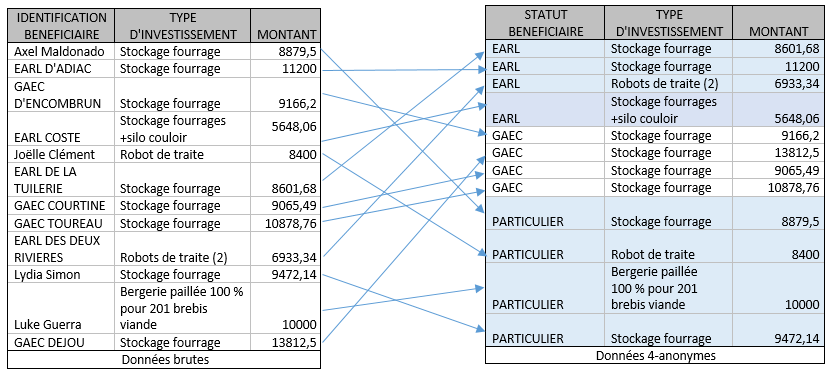
\includegraphics[width=1\textwidth]{images/anonymisation/k_anonym_image1.png}
    \caption{Exemple d'une k-anonymisation : données 4-anonymes}
    \label{Exemple d'une k-anonymisation : données 4-anonymes}
\end{figure}


\paragraph{Evaluation du k-anonymat:}  
\begin{itemize}
    \item \textbf{Individualisation :} étant données les classes d’équivalence, nous savons qu’au moins k individus partagent certains attributs dans le jeu de données. Il ne devrait plus être possible d’isoler un individu dans un groupe de k autres individus. 

    \item \textbf{Corrélation:} il est possible de relier les enregistrements par groupe de k-individus. Au sein d’un même groupe, la probabilité que deux enregistrements correspondent à un individu est de 1/k. 

    \item \textbf{Inférence:} si tous les k individus d’une classe d’équivalence ont la même valeur pour un attribut donné et que cette information est sensible, il suffit de connaître à quelle classe d’équivalence appartient un individu pour déduire sa données sensible. 
\end{itemize}
 
Alors que k-anonymat protège contre la divulgation d'identité, il n'offre pas une protection suffisante contre la divulgation d'attributs. Cela a été reconnu par plusieurs auteurs[13], [14]. Deux attaques ont été identifiées dans: attaque d'homogénéité et l'attaque de connaissances de fond[14]. 
\subsection{L-diversité}
%ajout d'exeple

La l-diversité est une technique d’agrégation qui étend la k-anonymisation. En effet, il est toujours possible de déduire les informations sensibles si les k individus d’une classe d’équivalence possèdent tous la même information sensible Figure \ref{fig:Données 3-anonymes mais pas l-diverses}

La l-diversité ajoute une contrainte selon laquelle les k-enregistrements d’une classe d’équivalence doivent avoir au minimum l valeurs distinctes comme dans la figure \ref{fig:Données 3-anonymes et 3-diverses}

%ajout d'exemple

Dans l’exemple \ref{fig:Données 3-anonymes mais pas l-diverses}, si l’on sait qu’une personne cultive une grande culture (blé, mais, orge) on déduit quel type de pesticides elle utilise, dans notre cas, les fongicides (\textbf{\textbf{homogeneity Attack}}).  Comme citer en haut, l’inférence est la grande faiblesse du k-anonymat.La l-diversité vient y remédier en y ajout une contrainte Figure \ref{fig:Données 3-anonymes et 3-diverses}. 

Ainsi donc on n’est plus en mesure de deviner le type de pesticides utilisé en fonction du type de culture.  

Cependant, avec une attaque d’inférence probabiliste, on peut par exemple déduire avec une certaine probabilité assez élevée, le type de pesticide utilisé. En effet, si la personne malveillante sait qu’Alan, qui est la seule personne à avoir une parcelle de 38ha, alors, il lui est possible de deviner, avec une probabilité de 1/3, le type de pesticide qu’Alan utilise (\textit{\textbf{Background Knowledge Attack}}). \cite{nguyen_techniques_2014}
\begin{figure}[!h]
    \centering
      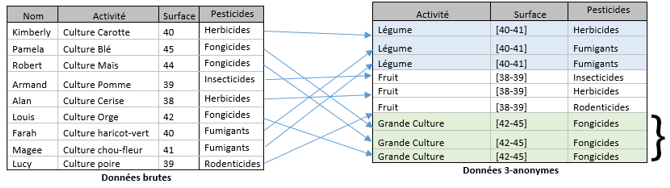
\includegraphics[width=1\textwidth]{images/anonymisation/l_divers_image1.png}
    \caption{ Données 3-anonymes mais pas l-diverses}
     \label{fig:Données 3-anonymes mais pas l-diverses}
   
\end{figure}


\begin{figure}[!h]
    \centering
      
   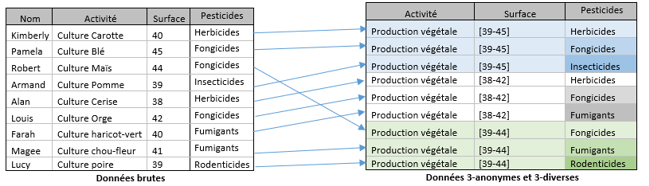
\includegraphics[width=1\textwidth]{images/anonymisation/l_divers_image2.png}
    \caption{Données 3-anonymes et 3-diverses }
     \label{fig:Données 3-anonymes et 3-diverses}
\end{figure}

\paragraph{Évaluation de L-diversité : }
\begin{itemize}
    \item \textbf{Individualisation:} la l-diversité empêche que les enregistrements relatifs à un individu soient isolés dans la base de données 

   \item \textbf{Corrélation:} la l-diversité n’apporte pas d’amélioration par rapport au k-anonymat.  

   \item \textbf{Inférence:} bien qu’il ne soit plus possible de faire des attaques par inférence, il reste cependant possible de mener des attaques par inférence probabiliste. 
\end{itemize}



\subsection{T-proximité}
La t-proximité formalise l’idée de la connaissance globale en exigeant que la distribution d’un attribut sensible soit, pour toute classe d'équivalence, proche de sa distribution dans l’ensemble du jeu de données. 
\section{les Techniques de généralisation}
\subsection{La permutation}
Aussi appelé désalignement, ou shuffling, elle consiste à échanger les positions des données dans un jeu de données. En d’autres mots, c’est-à-dire que les données sont là mais pas à la bonne place. Elle est utile quand il est important de conserver la distribution exacte de chaque attribut dans l’ensemble de données. Si deux ou plusieurs attributs sont liés par une relation logique ou une corrélation statique et sont permutés indépendamment l’un de l’autre, ce lien sera détruit [4]. 

\begin{figure}[!h]
    \centering
     \label{exemple d'une permutation}
    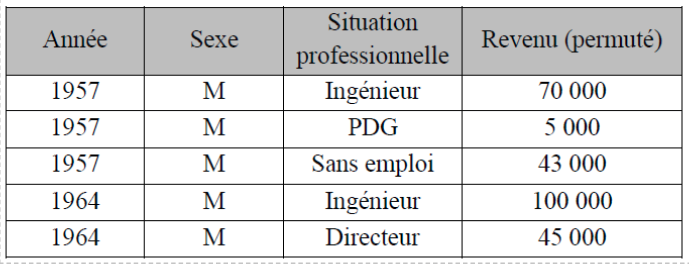
\includegraphics[width=1\textwidth]{images/anonymisation/permutation_image1.png}
    \caption{exemple d'une permutation}
   
\end{figure}
\paragraph{Evaluation de la permutation : }
\begin{itemize}
    \item \textbf{Corrélation:} si la permutation affecte des attributs et des quasi-identifiants, elle peut empêcher de relier «correctement» des attributs entre eux tant à l’intérieur qu’à l’extérieur d’un ensemble de données, mais elle autorise toujours une corrélation «incorrecte» puisqu’une entrée réelle peut se trouver associée à une personne concernée différente. 

    \item \textbf{Inférence:} Des déductions peuvent encore être tirées de l’ensemble des données, en particulier si les attributs sont corrélés entre eux ou ont des relations logiques fortes; toutefois, sans savoir quels attributs ont été permutés, l’attaquant doit envisager la possibilité que son inférence se fonde sur une hypothèse et seule une inférence probabiliste demeure possible. 

Si les attributs sont liés par une forte relation logique, alors la permutation peut être détectée et peut même être inversée. 
\end{itemize}
\subsection{L’ajout de Bruit} 

L’ajout de bruit consiste à rendre moins précis un ensemble de données en ajoutant ou en retirant de l’information sur les enregistrements tout en conservant la distribution générale. Les enregistrements restent identifiables mais sont moins fiables [15]. 

L’ajout de bruit doit normalement être combiné à d’autres techniques d’anonymisation pour être efficace\cite{noauthor_repertoire_2018-1}.  

\paragraph{Évaluation de l’ajout de bruit : }

\begin{itemize}
    \item  \textbf{Individualisation}: l’ajout de bruit n’empêche pas la possibilité d’une isolation. Même si l’enregistrement est moins fiable, il reste possible d’isoler tous les enregistrements concernant un individu. 
    
    \item  \textbf{Corrélation}: il est toujours possible de relier les enregistrements (issu d’un ou de plusieurs jeux de données différents) d’un même individu. 
    
    \item \textbf{Inférence}: le taux de succès avec une attaque par inférence est beaucoup moins élevé. 
\end{itemize}

\paragraph{Erreurs courantes}:   
\begin{itemize}
    \item Ajout de bruit incohérent : si le bruit ne respecte pas la logique des attributs ou si celui-ci est disproportionné, on peut alors imaginer qu'un attaquant puisse identifier le bruit, le filtrer et ainsi recréer un jeu de données. 
    \item supposer que l’ajout de bruit est suffisant : L'ajout de bruit n'est pas une technique qui se suffit. Pour être efficace, elle doit s'utiliser en complément avec d'autres techniques pour rendre difficile la récupération des données.
\end{itemize}


\subsection{La confidentialité différentielle}
%ajouter du texte sur la confidentialité confidentielle
La confidentialité différentielle est l'une des techniques les plus populaire ces dernières années surtout dans la recherche. En effet, contrairement aux autres techniques, elle est la seule à pouvoir fournir des preuves mathématiques sur la possibilité de borner l'information qui peut être appris sur un individus.

\subsubsection{Formalisation}
soit \begin{math}\epsilon\end{math} un réel et\begin{math}A\end{math} une algorithme probabiliste qui prend pour entrée un jeu de données. Soit \begin{math}imgA\end{math} image de \begin{math}A\end{math}. L'algorithme \begin{math}A\end{math} et dit \begin{math}\epsilon\end{math}-différentiellement confidentiel, si, pour tout jeux de données \begin{math}D_{1}\end{math} et \begin{math}D_{2}\end{math} qui diffèretnt d'une seul élément(l'information a propos d'une seule personne) et pour sous ensemlbe \begin{math}S\end{math} de \begin{math}imgA\end{math},

\[
Pr[A(D_{1})\in S] \leq e^{\epsilon} * Pr[A(D_{2})\in S]
\]
où la probabilité est fondés sur l'aléa introduit par l'algorithme. D'après cette définition, la confidentialité différentielle port sur l'algorithme lui-même, et non sur les données traitées.
\subsubsection{Exemple}
Soit une base de données médicale \begin{math}D_{1}\end{math}, dans laquelle chaque enregistrement contient deux informations \textbf{(Nom,X)} où X est un booléen qui indique si une personne a le diabète ou non.

On suppose qu'un utilisateur malintentionné veut connaître l'état de santé de Sophie. On suppose également qu'il connaît ligne qui correspond à Sophie(Ligne 5). L'utilisateur n'est autorisé à questionner la base qu'à travers d'une Fonction \begin{math}F_{i}\end{math} qui renvoie une somme des \begin{math}i\end{math} premiers lignes. Cet utilisateur peut connaître l'état de santé de Sophie en fesant un simple Différence entre \begin{math}F_{5}(D_{1}) = 3\end{math} et \begin{math}F_{4}(D_{1}) = 2\end{math}

En poursuivant avec cet exemple, si l'on construit maintenant une base D2 en remplaçant(Sophie,1) par (Sophie, 0) alors cet utilisateur sera capable de sitinguer \begin{math}D2\end{math} et \begin{math}D1\end{math} en calculat la différence \begin{math}F_{5} - F_{4}\end{math}. S'il était amnené à rececoir les valeurs \begin{math}F_{i}\end{math} via un algorithme \begin{math}\epsilon\end{math}-différentiellement confidentiel, pour un \begin{math}\epsilon\end{math} suffisamment peti, alors il serait incapable de faire la différence entre \begin{math}D_{2}\end{math} et \begin{math}D_{1}\end{math}.

\paragraph{Évaluation de la confidentialité différentielle}
\begin{itemize}
    \item \textbf{Individualisation:} si les résultats se limitent à la production de statistiques et si les règles appliquées à l’ensemble de données sont bien choisies, il ne devrait pas être possible d’utiliser les réponses pour isoler un individu. 

    \item \textbf{Corrélation:} en recourant à des requêtes multiples, il pourrait être possible de relier entre elles les entrées relatives à un individu spécifique d’une réponse à l’autre. 

    \item \textbf{Inférence:} il est possible de déduire des informations concernant des individus ou des groupes au moyen de requêtes multiples. 
\end{itemize}
\chapter{Conclusion}
Compte tenu de la réglementation actuelle, il y a obligation d'assurer une  confidentialité minimale  des données en général et des données à caractères personnelles en particulier. Il existe plusieurs méthodes et techniques qui assurent cette confidentialité mais le choix de celles-ci dépendra de la sensibilité des données ou des applications visées. Ce choix dépendra aussi de l'ensemble des moyens (techniques et financiers) raisonnablement susceptible d'être utilisé pour identifier une personne physique directement ou indirectement. Bien que le domaine agricole soit en retard par rapport au monde de la santé et de la finance en matière de protection des données, il est essentiel que celui-ci puisse vite se développer pour renforcer la confiance des producteurs nécessaire aux partages de leurs données et permettre ainsi de faire émerger de nouvelles connaissances et de nouveaux services.